\section{Experimental Evaluation}
\label{sec:exp}

\begin{figure*}[t]
\vspace{-0.2in}
\centering
\begin{minipage}{2.1in}
\centering
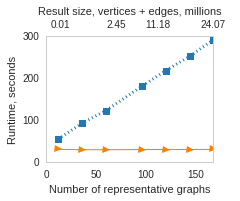
\includegraphics[width=2.1in]{figs/slice_wikitalk_build13.png}
\vspace{-0.2in}
\caption{Slice on wiki-talk.}
\label{fig:slicewiki}
\vspace{-0.1in}
\end{minipage}
\begin{minipage}{2.1in}
\centering
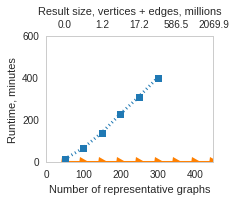
\includegraphics[width=2.1in]{figs/slice_ngrams_build13.png}
\vspace{-0.2in}
\caption{Slice on nGrams.}
\label{fig:slicengrams}
\vspace{-0.1in}
\end{minipage}
\begin{minipage}{2.1in}
\centering
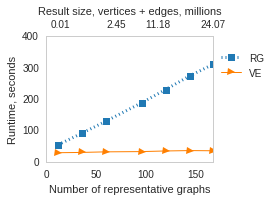
\includegraphics[width=2.4in]{figs/project_wikitalk_build13.png}
\vspace{-0.2in}
\caption{Map on wiki-talk.}
\label{fig:project}
\vspace{-0.1in}
\end{minipage}
\end{figure*}

\begin{figure*}[t!]
\centering
\begin{subfigure}{0.3\textwidth}
%\begin{minipage}{2.2in}
%\centering
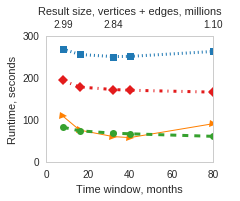
\includegraphics[width=2.2in]{figs/agg_allall_wikitalk_build13.png}
\caption{$Q_V=\insql{all}$, $Q_E=\insql{all}$, wiki-talk}
%\caption{Aggregate by time, all/all quantification on the wiki-talk dataset.}
\label{fig:agg1}
%\end{minipage}
\end{subfigure}
\begin{subfigure}{0.3\textwidth}
%\begin{minipage}{2.2in}
%\centering
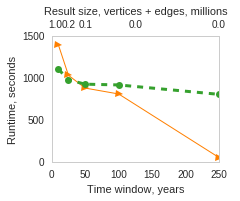
\includegraphics[width=2.2in]{figs/agg_allexists_ngrams_build13.png}
\caption{$Q_V=\insql{all}$, $Q_E=\insql{exists}$, nGrams}
%\caption{Aggregate by time, all/exists quantification on the nGrams dataset.}
\label{fig:agg2}
%\end{minipage}
\end{subfigure}
\begin{subfigure}{0.36\textwidth}
%\begin{minipage}{2.5in}
%\centering
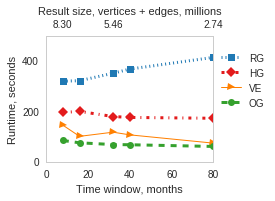
\includegraphics[width=2.5in]{figs/agg_allexists_wikitalk_build13.png}
\caption{$Q_V=\insql{all}$, $Q_E=\insql{exists}$, wiki-talk}
%\caption{Aggregate by time, all/exists quantification on the wiki-talk dataset.}
\label{fig:agg4}
%\end{minipage}
\end{subfigure}
\vspace{-0.1in}
\caption[]{Aggregate by time.}
\vspace{-0.1in}
\label{fig:agg}
\end{figure*}

{\bf Experimental environment.} All experiments in this section were
conducted on a 16-slave in-house Open Stack cloud, using Linux Ubuntu
14.04 and Spark v2.0.  Each node has 4 cores and 16 GB of RAM.  Spark
Standalone cluster manager and Hadoop 2.6 were used.
%
Because Spark is a lazy evaluation system, a materialize operation was
appended to the end of each query, which consisted of the count of
nodes and edges.  Each experiment was conducted 3 times with a cold
start, we report the average running time, which is representative
because we took great care to control variability: standard deviation
for each measure is at or below 5\% of the mean except in cases of
very small running times.

OG and HG inherit their implementation of \insql{slice}, \insql{map}
and \insql{subgraph} from RG and are not included in these
experiments.  Performance of all 4 data structures is compared in
\insql{aggregation}, \insql{union} and \insql{intersection}.

{\bf Data.}  We evaluate performance of our framework on three real
open-source datasets, summarized in Table~\ref{tab:datasets}.
wiki-talk (\url{http://dx.doi.org/10.5281/zenodo.49561}) contains over
10 million messaging events among 3 million wiki-en users\eat{2002
  through 2015}, aggregated at 1-month resolution.\\nGrams
(\url{http://storage.googleapis.com/books/ngrams/books/datasetsv2.html})
contains word co-occurrence pairs\eat{ from 1520 through 2008}, with
30 million word nodes and over 2.5 billion undirected edges.  The
Twitter social graph~\cite{Gabielkov:2014:SSN:2591971.2591985}
contains over 23 billion directed follower relationships between 0.5
billion twitter users\eat{ collected in 2012}, sampled at 1-month
resolution.\eat{ based on account creation information from April
  2006.} \eat{DELIS contains monthly snapshots of a portion of the Web
  graph focusing on the .uk domains from 05/2006 through
  05/2007~\cite{BSVLTAG}. }The datasets differ in size, in the number
and type of attributes and in evolution rates, calculated as the
average graph edit similarity~\cite{Ren2011}. \eat{the evolutionary
  properties: co-authorship network nodes and edges have limited
  lifespan, while the nGrams network grows over time, with nodes and
  edges persisting for long duration.  All figures in the body of this
  section are on the larger nGrams dataset.  Refer to the Appendix for
  the DBLP figures, which show similar trends as nGrams.}

\eat{The behavior of the four physical representations reported below is
dependent on the underlying data format on disk
(Section~\ref{sec:sys:maint}), and should be interpreted in that
context.}

{\bf Slice} performance was evaluated by varying the slice time window
and materializing the \tg, and is presented in
Figures~\ref{fig:slicewiki} for wiki-talk and~\ref{fig:slicengrams}
for nGrams.  Similar trends were observed for twitter.  Slice is
expected to be more efficient when executed over VE when data is
coalesced on disk than over \sg, and we observe this in our
experiments.  This is because multiple passes over the data are
required for \sg to compute each representative graph, leading to
linear growth in running times for file formats and systems without
filter pushdown, as is the case here.  Slice over VE simply execute
temporal selection and has constant running times (29 sec for
wiki-talk, about 1.5 min for nGrams).\eat{Recall that in VE
  \insql{slice} performs temporal selection, and method when data on
  disk is coalesced.  \sg, in contrast, does multiple passes of select
  over the same data to compute each RG.  Thus, as expected, VE
  behavior is directly dependent on the size of input data regardless
  of the slice size for file formats and systems without filter
  pushdown, as is the case here, or if the data does not have temporal
  locality (Figure~\ref{fig:slicewiki}, Figure~\ref{fig:slicengrams}
  -- about 1.5 minutes for VE).  \sg behavior is linear in the slice
  size. } This experiment essentially measures the cost of
materializing \sg from a \ve on-disk representation.  We observed the
same linear trend in our preliminary work, when the data was stored as
individual snapshots on disk, although less redundant work is needed
in that case.

\eat{
\begin{figure*}[th]
\centering
\begin{minipage}{2.2in}
\centering
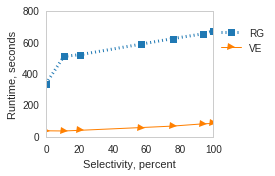
\includegraphics[width=2.2in]{figs/subgraph_wikitalk_build13.png}
\caption{Subgraph on wiki-talk.}
\vspace{-0.1in}
\label{fig:subgraphwiki}
\vspace{-0.1in}
\end{minipage}
\begin{minipage}{2.2in}
\centering
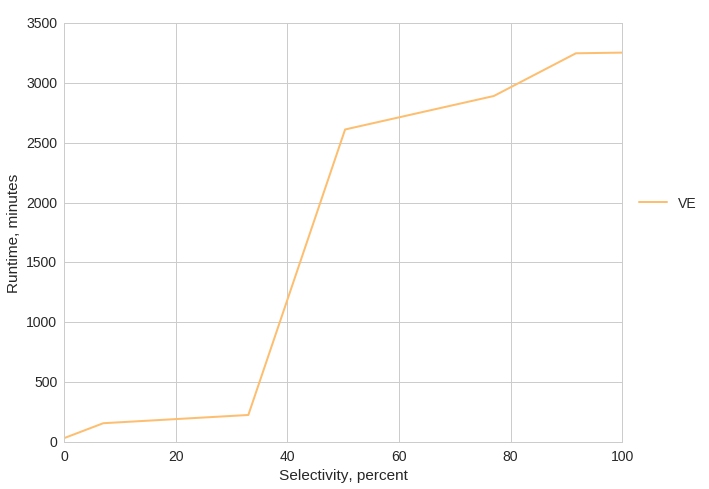
\includegraphics[width=2.2in]{figs/select_ngrams_edges_build12.png}
\vspace{-0.1in}
\caption{Select on the nGrams dataset, return edges.}
\vspace{-0.1in}
\label{fig:subgraphngrams}
\end{minipage}
\end{figure*}
}

{\bf Map}\eat{ We evaluate \insql{map} performance by varying the data
  size through the \insql{slice} operation.} exhibits a similar trend
as \insql{slice}: constant running time for VE and a linear increase
in running time with increasing number of representative graphs for
\sg (Figure~\ref{fig:project} for wiki-talk, similar for other
datasets).  Performance of \insql{map} is slightly worse than that of
\insql{slice} because \insql{map} must coalesce its output as the last
step, while \insql{slice} does not. 

{\bf Subgraph} performance was evaluated by specifying a condition on
the $length(a.attr)<t$ of the vertex attribute, with different values
of $t$ leading to different selectivity.  This experiment was executed
for wiki-talk (with $username$ as the attribute) and for nGrams (with
$word$ as the attribute).  Twitter has no vertex attributes and was
not used in this experiment.  Performance on \sg is a function of the
number of intervals and is insensitive to the selectivity
(Figure~\ref{fig:subgraphngrams} for nGrams, similar for wiki-talk).
The behavior on VE is dominated by FK enforcement: with high
selectivity (few vertices) broadcast join affords performance linear
in the number of edges, whereas for a large number of vertices
broadcast join is infeasible and a hash-join is used instead, which is
substantially slower.  VE provides an order of magnitude better
performance than \sg: up to 3 min with hash-join and up to 15 min with
broadcast join for VE, in contrast to between 95 and 200 min for \sg.

\begin{table}
\caption{Experimental datasets.}
\vspace{-0.1in}
\small
\begin{tabular}{l | c | c | c | c }
\hline
\multicolumn{1}{l|}{\bfseries Dataset} & \multicolumn{1}{c|}{\bfseries |V|} & \multicolumn{1}{c|}{\bfseries |E|} & \multicolumn{1}{c|}{\bfseries Time Span} & \multicolumn{1}{c}{\bfseries Evol. Rate} \\ \hline
wiki-talk-en & 2.9M & 10.7M & 2002--2015 & 14.4 \\ \hline
nGrams & 29.3M & 2.5B & 1520--2008 & 16.67 \\ \hline
%%DELIS & 128M & 40.5B & 2006--2007 & ? \\ \hline
twitter & 505.4M & 23B & 2006--2012 & 88 \\ \hline
\end{tabular}
\vspace{-0.1cm}
\label{tab:datasets}
\end{table}

\begin{figure*}[t]
\begin{minipage}{2.1in}
\centering
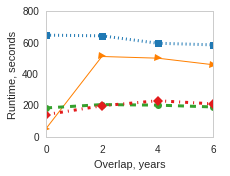
\includegraphics[width=2.1in]{figs/union_wikitalk_build13.png}
\vspace{-0.2in}
\caption{Union on wiki-talk.}
\label{fig:union1}
\vspace{-0.1in}
\end{minipage}
\begin{minipage}{2.1in}
\centering
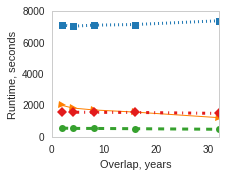
\includegraphics[width=2.1in]{figs/union_ngrams_build13.png}
\vspace{-0.2in}
\caption{Union on nGrams.}
\label{fig:union2}
\vspace{-0.1in}
\end{minipage}
\begin{minipage}{2.2in}
\centering
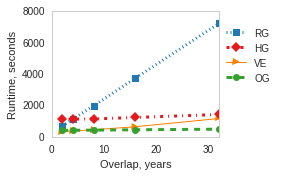
\includegraphics[width=2.55in]{figs/intersect_ngrams_build13.png}
\vspace{-0.2in}
\caption{Intersection on nGrams.}
\label{fig:intersectngrams}
\vspace{-0.1in}
\end{minipage}
\end{figure*}

\begin{figure*}[t]
\centering
\begin{minipage}{2.2in}
\centering
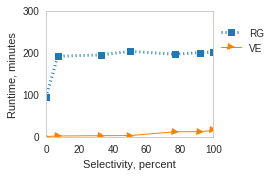
\includegraphics[width=2.2in]{figs/subgraph_ngrams_build13.png}
\vspace{-0.2in}
\caption{Subgraph on nGrams.}
\label{fig:subgraphngrams}
\vspace{-0.1in}
\end{minipage}
\begin{minipage}{2.15in}
\centering
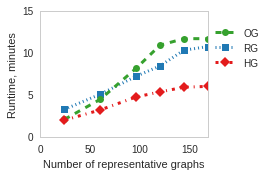
\includegraphics[width=2.15in]{figs/cc_wikitalk_build13.png}
\vspace{-0.2in}
\caption{Components on wiki-talk.}
\label{fig:ccwiki}
\vspace{-0.1in}
\end{minipage}
\begin{minipage}{2.2in}
\centering
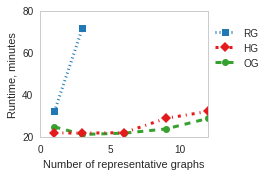
\includegraphics[width=2.2in]{figs/prank_twitter_build13.png}
\vspace{-0.2in}
\caption{PageRank on Twitter.}
\label{fig:pranktwitter}
\vspace{-0.1in}
\end{minipage}
\end{figure*}

{\bf Aggregation} performance was evaluated on 4 representations,
since all have different implementations of this operator.  We
executed structure-only aggregation (no attributes), varying the size
of the aggregation window.  We observed that performance depends
heavily on the quantification, and on the data evolution rate.  \og is
an aggregated data structure with good temporal locality and thus in
most cases provides good performance and is insensitive to the
aggregation window size (Figure~\ref{fig:agg1}).  However, in datasets
with a large number of representative graphs (such as nGrams), \og is
slow on large windows, an order of magnitude worse than VE
(Figure~\ref{fig:agg2}).  VE outperforms \og when vertex and edge
quantification levels match (Figure~\ref{fig:agg1}), but is worse than
\og when vertex quantification is stricter than edge quantification
and FK must be enforced (Figure~\ref{fig:agg4}).  \og also outperforms
VE when both evolution rate is low and aggregation window is small
(Figure~\ref{fig:agg1}, wiki-talk).\eat{ \sg and \hg do not provide
  the best performance on any of our datasets.}

{\bf Union and intersection} by structure was evaluated by loading two
time slices of the same dataset with varying overlap.  Performance
depends on the size of the overlap (in the number of representative
graphs) and on the evolution rate.  VE has best performance when
overlap is small (Figure~\ref{fig:union1})\eat{ and when the evolution
  rate is high (Figure~\ref{fig:union2}), regardless of the size of
  the overlap}.  \og always has good performance, constant
w.r.t. overlap size.  This is expected, since \og \insql{union} and
\insql{intersection} are implemented as joins (outer or inner) on the
vertices and edges of the two operands.  VE, on the other hand, splits
the coalesced vertices/edges of each of the two operands into
intervals first, takes a union, and then reduces by key.  When
evolution rate is low and duration of an entity is high, such as in
wiki-talk for vertices, the split produces a lot of tuples to then
reduce, and the performance suffers (Figure~\ref{fig:union1}). \sg
only has good performance on \insql{intersection} when few
representative graphs overlap, and never on \insql{union}
(Figure~\ref{fig:intersectngrams}). \hg performance is generally worse
than \og, by a constant amount in \insql{union}, and diverges in
\insql{intersection}.

{\bf Analytics.}  We implemented PageRank (PR) and Connected
Components (CC) analytics for the three graph-based representations
using the Pregel GraphX API.  PR was executed for 10 iterations or
until convergence, whichever came first. CC was executed until
convergence with no limit on the number of iterations.  Performance of
Pregel-based algorithms depends heavily on the partitioning strategy,
with best results achieved where cross-partition communication is
small~\cite{MoffittTempWeb16}.  For this reason, we evaluated only
with the E2D strategy.
%
Performance was evaluated on time slices of varying size.  For a very
small number of graphs (1-2), \sg provides good performance, but slows
down linearly as the number of graphs increases.  \hg provides the
best performance on analytics under most conditions, with a linear
increase but a significantly slower rate of growth.  The tradeoff
between \og and \hg depends on graph evolution characteristics.  If
the graph is a growth-only evolution (such as in Twitter), \og is not
denser than \hg and computes everything in a single batch, which leads
to the fastest performance, as can be seen in
Figure~\ref{fig:pranktwitter}.  If the edge evolution represents more
transient connections, then \hg is less dense and scales better
(Figure~\ref{fig:ccwiki}).  Note that \og and \hg performance could be
further improved by computing them over coalesced structure-only V and
E, and ignoring attributes.

{\bf Cluster Size.}  We next examine how the system performance scales
with the size of the cluster.  We execute
\insql{slice; aggregate(1 year, exists, exists); components}.
%
\eat{
\begin{small}
\begin{verbatim}
   slice
   aggregate(1 year, exists, exists)
   connected components
   materialize vertices
\end{verbatim}
\end{small}
}
This query, executed on the wiki-talk dataset, computes connected
components over the past 10 years on the yearly scale.  Over the
twitter dataset the slice size is 2 years.

%%\begin{small}
%%\begin{verbatim}
%%Q2. UKDELIS
%%
%%   aggregate(3 months, exists, always)
%%   pagerank(20 iterations)
%%   project pagerank score
%%   aggregate(12 months, exists, exists, trend)
%%   get top 10
%%\end{verbatim}
%%\end{small}
\eat{
This query, executed on DELIS dataset, computes stable links between
websites, i.e. links that persist for 3 months, and uses them to
compute pagerank for each.  The score is projected and its trend
computed in an aggregation over the whole dataset time period (1
year).  The top 10 websites with the highest increase in pagerank are
returned.
}

The best performing representation was selected based on our
experimental results.  Slice, project, and aggregate were performed
with VE, analytics with \hg.  The results are in
Table~\ref{tab:clustersize}.  Both queries show improvements in
running time as the cluster size grows, with diminishing returns.
\eat{With the small wiki-talk dataset, performance improves initially
  with larger cluster sizes but levels off at the largest size.  With
  the large twitter dataset, ...}

\begin{table}
\centering
\caption{Effect of cluster size, minutes.}
\vspace{-0.1in}
\small
\begin{tabular}{| l | c | c | c | c |}
\hline
\multicolumn{1}{|l|}{\bfseries Dataset} & \multicolumn{1}{c|}{\bfseries 4 slaves} & \multicolumn{1}{c|}{\bfseries 8 slaves} & \multicolumn{1}{c|}{\bfseries 12 slaves} & \multicolumn{1}{c|}{\bfseries 16 slaves}\\ \hline
wiki-talk & 8.41 & 6.02 & 5.02 & 2.94 \\ \hline
Twitter & 151.77 & 72.75 & 55.68 & 53.46 \\ \hline
\end{tabular}
\label{tab:clustersize}
\end{table}

{\bf In summary,} no one data structure is most efficient across all
operations.  VE provides the best performance for slice, map, and
subgraph.  \og is efficient for aggregation under most conditions, and
\hg for analytics.  The graph evolution rate is an important factor in
selecting the more suitable representation.
